\chapter{Iteración 7: Implementación de un sistema de gestión para la placa de instrumentación} % (fold)
\label{cha:iteracion_7}

\section{Introducción} % (fold)
\label{it7:sec:introduccion}

Hasta el momento, utilizamos una computadora de uso común para que configure el sistema y haga uso de sus funcionalidades. Pero, uno de los objetivos del proyecto es que sea un sistema embebido de un uso mas especifico el que realice estas acciones a la plataforma. Con esto en mente, consideramos que es necesario comprobar el funcionamiento del sistema con algún embebido que tome la función de recibir los datos de telemetría y controlar la plataforma.

La implementación de este sistema embebido estará orientada al uso y control de la plataforma, y en particular, al control del sensor de campo electrostático con el que se trabajo en la iteración anterior. De esta forma, obtendremos una prueba de campo similar a un producto final.

El objetivo principal es correr un programa en un sistema embebido, que se comunique con la plataforma de instrumentación, sea capaz de configurarla, y tener acceso directo a las funcionalidades ligadas al sensor de campo electrostático.

El programa sera desarrollada basándonos en partes del proyecto integrador de Gaston Lucero. El proyecto de Lucero consiste en un sistema gestionador de dispositivos IoT. Parte del software de gestión es un servidor web desarrollado en python, que es posible de embeber en una placa de desarrollo y actuar como el sistema gestionador al que se le envían los datos de telemetría. En esta iteración, trabajaremos sobre este software, intentando adaptarlo al uso con nuestra plataforma, con el fin de cumplir con los objetivos de la iteración.

% section introduccion (end)

\section{Requerimientos de la iteración} % (fold)
\label{it7:sec:requerimientos_de_la_iteracion}

Al igual que en la iteracion anterior, los requerimientos no son especificos de la plataforma, sino de un sistema anexo que trabaja con la misma. En este caso, listamos los requerimientos de un sistema de gestion que cumplira el papel de controlar la plataforma de instrumentacion.

\begin{itemize}
\item Parte del software de gestion deberia ser un servidor web con conexion a internet e interfaz grafica de usuario. [6.1]
\item Mediante una interfaz grafica HTML, se deberian poder realizar las mismas configuraciones que permite la interfaz de linea de comando de la plataforma. [6.2]
\item Se deberían guardar datos de mediciones e información que se considere importante en una base de datos local, accesible vía la interfaz web gráfica. [6.3]
\item Debería permitir establecer intervalos de fecha, hora y minuto para medir campo electrostático en los canales 0 y 1 de la plataforma en modo diferencial. [6.4]
\item La conexión entre el sistema de gestion y un dispositivo manejado por el usuario (computadora con conexión a internet, smartphone) debería ser vía Wi-Fi. [6.5]
\end{itemize}

% section requerimientos_de_la_iteracion (end)


\section{Placa de desarrollo elegida para la implementación} % (fold)
\label{it7:sec:placa_de_desarrollo_elegida_para_la_implementacion}

Teniendo en cuenta los requerimientos, listamos una serie de requisitos que debe cumplir la placa de desarrollo que se seleccione:

\begin{itemize}
  \item Debería poder albergar un sistema operativo basado en Linux o Unix
  \item Debería permitir la conexión de un adaptador Wi-Fi USB
  \item Debería tener interfaz serial UART
\end{itemize}

Por cubrir con todos los requerimientos y por razones de disponibilidad, decidimos implementar este sistema en una placa de desarrollo Raspberry Pi B+ (figura \ref{fig:raspberrypi}), embebida con un sistema operativo Raspbian (Debían para Raspberry). Esta placa de desarrollo cumple con todos los requisitos mencionados anteriormente, por lo que es posible cubrir todos los requerimientos del sistema de gestión.

\begin{figure}[h]
  \centering
  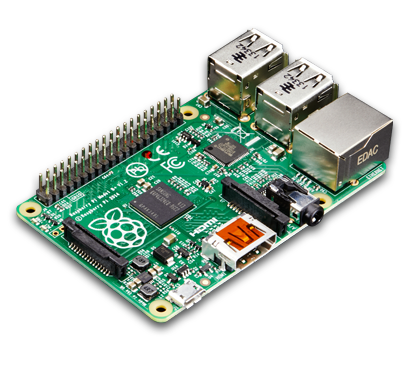
\includegraphics[width=0.80\textwidth, height = 7cm]{raspberrypi.png}
  \caption{Placa de desarrollo Raspberry Pi B+}\label{fig:raspberrypi}
\end{figure}
% section placa_de_desarrollo_elegida_para_la_implementacion (end)

\section{Diagramas de bloques} % (fold)
\label{it7:sec:diagramas_de_bloques}

Como etapa inicial del desarrollo, procedemos a graficar diagramas de bloques que describen el diseño estático del sistema.

\begin{figure}[h]
  \centering
  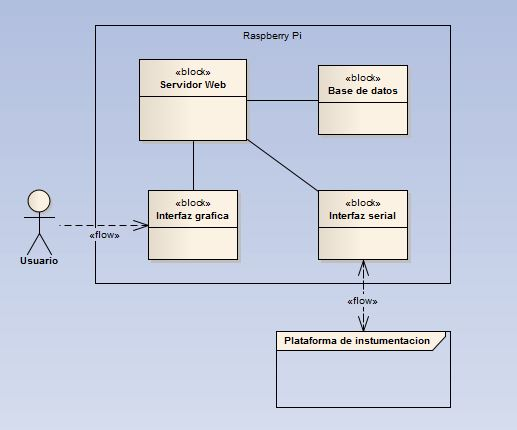
\includegraphics[width=0.80\textwidth, height = 7cm]{bloquessistemadegestion}
  \caption{Diagrama de bloques del sistema de gestión, implementado en una placa de desarrollo Raspberry Pi.}\label{fig:bloquessistemadegestion}
\end{figure}

\begin{figure}[h]
  \centering
  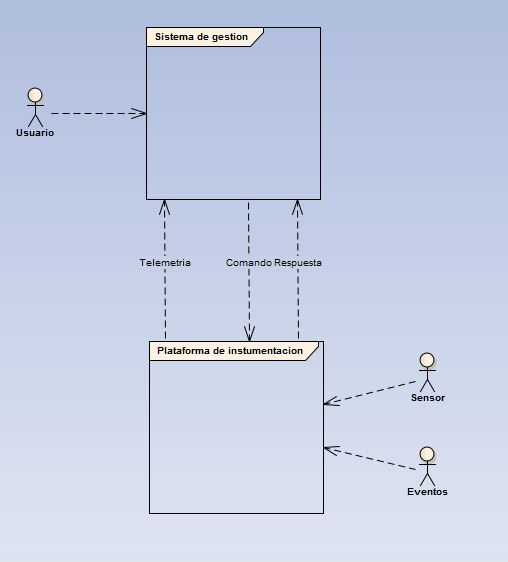
\includegraphics[width=0.80\textwidth, height = 7cm]{interaccionplataformaygestionador}
  \caption{Diagrama que ilustra la interacción entre la plataforma de instrumentación y el sistema gestionador}\label{fig:interaccionplataformaygestionador}
\end{figure}

La Figura \ref{fig:bloquessistemadegestion} muestra los distintos bloques del sistema de gestión y la figura \ref{fig:interaccionplataformaygestionador} ilustra la interaccion con la plataforma de instrumentación. El sistema esta compuesto por cuatro bloques básicos:

\begin{itemize}
  \item Una interfaz gráfica, que interactúa con el usuario
  \item Una interfaz serial, que interactúa con la plataforma de instrumentación
  \item Un bloque que maneja el sistema de gestión de una base de datos MySQL, para guardar la información de telemetría junto con los meta datos
  \item Un Servidor Web, que además de proveer conexión a internet, maneja los bloques mencionados.
\end{itemize}


% section diagramas_de_bloques (end)

\section{Servidor web} % (fold)
\label{it7:sec:servidor_web}

El servidor web fue desarrollado con ayuda de BottlePy. BottlePy es un Web Framework liviano, simple y rápido, sin otra dependencia que la librería estándar de Python. Incluye un servidor web HTTP, soporta mapeo de funciones a direcciones URL, y tiene un motor de generación de documentos HTML en base a templates programadas en Python.

Con el uso de este servidor, disponemos una conexión al servidor en una dirección IP fija dentro de una red LAN. Con un modulo Wi-Fi USB conectado a la placa Raspberry Pi, es posible tener conexión a una red LAN. Si un usuario de la misma red se conecta al puerto 80 (HTTP) de esa dirección IP en un navegador, podra visualizar la interfaz gráfica del servidor, y asi interactuar con el sistema de forma remota.

Al servidor web realizado por Lucero, también hecho con uso de BottlePy, se le realizo una adaptación hacia nuestros requerimientos. Se agregaron, modificaron y eliminaron funciones dentro del servidor web para orientarlo hacia nuestros objetivos. En particular, el cambio mas significativo fue agregarle una base de datos en MySQL, modificar la interfaz gráfica en HTML, y agregar la funcionalidad de los intervalos para mediciones con el sensor de campo electrostático.

% section servidor_web (end)

\subsection{Base de datos} % (fold)
\label{it7:sub:base_de_datos}

La base de datos fue desarrollada utilizando la librería ``MySQLdb'' de Python, especializada para uso de MySQL en servidores web.

Cuando se activa la conversión continua por medio del servidor, la base de datos guarda todos los datos entrantes y los clasifica según el modo de medición y el pin o los pines por donde se mide. Se guarda el valor de la medición y una marca de tiempo con fecha, hora, minuto y segundo; realizada con ayuda de internet, y con la marca de tiempo relativa proveniente de la plataforma.

SCREENSHOT DE LA BASE DE DATOS EN ACCION

% subsection base_de_datos (end)

\subsection{Interfaz grafica de usuario} % (fold)
\label{it7:sub:interfaz_grafica_de_usuario}

La interfaz gráfica proporciona al usuario un método mas amigable para la interacción con la plataforma, además de proveer algunas funcionalidades extra.

SCREENSHOTS DE LA INTERFAZ GRAFICA PARA EL MOTOR.

Desde esta interfaz, el usuario puede:

\begin{itemize}
  \item Enviar cualquiera de los comandos que pueda interpretar la plataforma, con sus correspondientes argumentos
  \item Medir de manera inmediata el pin 0 en modo canal único
  \item Encender/Apagar el motor del sensor de campo electrostático
  \item Establecer uno o varios intervalos de medición, con fecha y hora, donde el sensor de campo electrostático deberá encenderse, medir campo eléctrico, y enviar los datos a la Raspberry Pi.
\end{itemize}


% subsection interfaz_grafica_de_usuario (end)


\section{Pruebas} % (fold)
\label{it7:sec:pruebas}

\begin{table}[h]
\centering
\caption{Test de sistema 1: Configuración normal mediante la interfaz gráfica}
\label{it7:tab:testsistema1}
\begin{tabular}{p{2cm} p{9cm}}
\multicolumn{2}{c}{\cellcolor[HTML]{68CBD0}{\color[HTML]{000000} Prueba de sistema}} \\
Prueba \#        & 1 \\
\hline
Nombre           & Configuración normal mediante la interfaz gráfica \\                     
\hline
Requerimiento    & 6.1, 6.2, 6.5  \\
\hline
Descripción      & Se intentaran realizar configuraciones normales de la plataforma, mediante el uso de la interfaz gráfica del servidor web desarrollado \\
\hline
Pre-condiciones  & \tabitem Plataforma de instrumentación encendida y disponible para configurar  \\
                 & \tabitem Sistema de gestión en la placa Raspberry Pi levantado y conectado a la red local a una dirección IP fija \\
                 & \tabitem Ordenador con navegador abierto conectado via Wi-Fi a la dirección IP de la Raspberry Pi. Debería poder verse la interfaz gráfica del servidor \\
                 & \tabitem Raspberry Pi conectada a la placa de instrumentación mediante cable serial RS-232 \\
\hline

Post-condiciones & Los comandos deberían funcionar correctamente y de igual manera que si se ingresaran directamente en la plataforma de instrumentación  \\
\hline
Secuencia  & Ingresamos el comando ``SSE,0,1'' en la interfaz gráfica, y luego presionamos ``Enviar'' \\
\hline
Resultados       & La respuesta de la plataforma fue la respuesta exitosa del comando, indicando que se configuro el pin 0 en modo canal único, con un intervalo de 1. \\
\end{tabular}
\end{table}


\begin{table}[h]
\centering
\caption{Test de sistema 2: Intervalos de medición}
\label{it7:tab:testsistema2}
\begin{tabular}{p{2cm} p{9cm}}
\multicolumn{2}{c}{\cellcolor[HTML]{68CBD0}{\color[HTML]{000000} Prueba de sistema}} \\
Prueba \#        & 1 \\
\hline
Nombre           & Intervalos de medición \\                     
\hline
Requerimiento    & 6.4  \\
\hline
Descripción      & Verificar la funcionalidad de los intervalos de medición para el sensor de campo electrostático \\
\hline
Pre-condiciones  & \tabitem Plataforma de instrumentación encendida y disponible para configurar  \\
                 & \tabitem Sistema de gestión en la placa Raspberry Pi levantado y conectado a la red local a una dirección IP fija \\
                 & \tabitem Ordenador con navegador abierto conectado a la dirección IP de la Raspberry Pi. Debería poder verse la interfaz gráfica del servidor \\
                 & \tabitem Raspberry Pi conectada a la placa de instrumentación mediante cable serial RS-232 \\
                 & \tabitem Circuito de adaptación del sensor alimentado \\
                 & \tabitem Sensor apagado\\
\hline

Post-condiciones & El motor debería encenderse, medir durante el tiempo que dure el intervalo, enviar los datos por protocolo serial a la Raspberry Pi, y apagarse cuando finalice el tiempo del intervalo   \\
\hline
Secuencia  & \tabitem a las 15:00 hs, establecimos un intervalo entre las 15:01 y las 15:05, dando un total de 4 minutos de medición. \\
\hline
Resultados       & A las 15:01, se inicio la secuencia de arranque del motor, y luego de eso comenzó a enviar los datos de telemetría. Comprobamos que ningún eslabón fallaba al perturbar el campo eléctrico del sensor y verificar que los datos en la base de datos se correspondían con estas perturbaciones.
\end{tabular}
\end{table}

\begin{table}[h]
\centering
\caption{Test de sistema 3: Almacenamiento de informacion en la base de datos}
\label{it7:tab:testsistema3}
\begin{tabular}{p{2cm} p{9cm}}
\multicolumn{2}{c}{\cellcolor[HTML]{68CBD0}{\color[HTML]{000000} Prueba de sistema}} \\
Prueba \#        & 1 \\
\hline
Nombre           & Almacenamiento de informacion en la base de datos \\                     
\hline
Requerimiento    & 6.3  \\
\hline
Descripción      & Verifica que la informacion acerca de los comandos enviados, el reporte de errores y los datos de mediciones se guarden correctamente en la base de datos del servidor web\\
\hline
Pre-condiciones  & \tabitem Plataforma de instrumentación encendida y midiendo en conversiones continuas sobre un canal configurado en modo unico, con una fuente de tension conectada y encendida con un valor de 1.5 Volts  \\
                 & \tabitem Sistema de gestión en la placa Raspberry Pi levantado y conectado a la red local a una dirección IP fija \\
                 & \tabitem Ordenador con navegador abierto conectado a la dirección IP de la Raspberry Pi. Debería poder verse la interfaz gráfica del servidor \\
                 & \tabitem Raspberry Pi conectada a la placa de instrumentación mediante cable serial RS-232 \\
\hline

Post-condiciones & Al abrir las tablas, deberian verse los datos de conversion, los reportes de errores y los comandos enviados para la configuracion.   \\
\hline
Secuencia  & \tabitem Se da fin a la conversion continua. \\
           & \tabitem Se abre la pestaña de la interfaz grafica correspondiente a las tablas de la base de datos. \\
\hline
Resultados       & Los datos aparecian correctamente almacenados en la base de datos. (Figura \ref{basededatosfuncionando}) \\
\end{tabular}
\end{table}

\begin{figure}[h]
  \centering
  \includegraphics[width=0.80\textwidth, height = 7cm]{basededatosfuncionando}
  \caption{Captura de pantalla de las tablas de la base de datos, con la informacion de las mediciones, los comandos enviados, y los reportes de errores} \label{fig:basededatosfuncionando}
\end{figure}

% section pruebas (end)

\section{Conclusiones} % (fold)
\label{it7:sec:conclusiones}

Desde un punto de vista conceptual, esta ultima iteración fue realizada con el objetivo de generar abstracción entre los distintos sistemas. El servidor web que se ejecuta en la Raspberry Pi tiene la función de traducir acciones sobre una interfaz, en comandos, sobre otra interfaz; además de otras funciones adicionales. La plataforma de instrumentación fue diseñada de tal manera de permitir facilidad a la hora de diseñar un sistema de gestión que la controle. Los comandos y las respuestas son cadenas estructuradas de caracteres; esto amplia la cantidad de sistemas embebidos compatibles con nuestra plataforma. Así, se verifica que se cumple con uno de los requerimientos no funcionales de la plataforma: Portabilidad.

Al finalizar esta iteración, quedaron algunas partes sin concluir, en lo que respecta al servidor web en la Raspberry Pi. Pero, los requerimientos principales fueron cumplidos, a pesar de las limitaciones del servidor web desarrollado.
A pesar de esto, logramos obtener un prototipo de producto que puede ser considerado como un detector inteligente de campo electrostático. Partiendo de la plataforma de instrumentación, junto con el sensor y el servidor web en la Raspberry Pi, es posible que este prototipo evolucione a convertirse en un producto real.


% section resultados (end)

% chapter iteracion_7 (end)